% ----------------------------------------------------
% DAB: Processing Chain Design
% ----------------------------------------------------
\documentclass[class=report,11pt,crop=false]{standalone}
% Page geometry
\usepackage[a4paper,margin=20mm,top=25mm,bottom=25mm]{geometry}

% Font choice
\usepackage{lmodern}

% Use IEEE bibliography style
\bibliographystyle{IEEEtran}

% Line spacing
\usepackage{setspace}
\setstretch{1.20}

% Ensure UTF8 encoding
\usepackage[utf8]{inputenc}

% Language standard (not too important)
\usepackage[english]{babel}

% Skip a line in between paragraphs
\usepackage{parskip}

% For the creation of dummy text
\usepackage{blindtext}

% Math
\usepackage{amsmath}

% Header & Footer stuff
\usepackage{fancyhdr}
\pagestyle{fancy}
\fancyhead{}
\fancyhead[R]{\nouppercase{\rightmark}}
\fancyfoot{}
\fancyfoot[C]{\thepage}
\renewcommand{\headrulewidth}{0.0pt}
\renewcommand{\footrulewidth}{0.0pt}
\setlength{\headheight}{13.6pt}

% Epigraphs
\usepackage{epigraph}
\setlength\epigraphrule{0pt}
\setlength{\epigraphwidth}{0.65\textwidth}

% Colour
\usepackage{color}
\usepackage[usenames,dvipsnames]{xcolor}

% Hyperlinks & References
\usepackage{hyperref}
\definecolor{linkColour}{RGB}{77,71,179}
\hypersetup{
    colorlinks=true,
    linkcolor=linkColour,
    filecolor=linkColour,
    urlcolor=linkColour,
    citecolor=linkColour,
}
\urlstyle{same}

% Automatically correct front-side quotes
\usepackage[autostyle=false, style=ukenglish]{csquotes}
\MakeOuterQuote{"}

% Graphics
\usepackage{graphicx}
\graphicspath{{Images/}{../Images/}}
\usepackage{makecell}
\usepackage{transparent}

% SI units
\usepackage{siunitx}

% Microtype goodness
\usepackage{microtype}

% Listings
\usepackage[T1]{fontenc}
\usepackage{listings}
\usepackage[scaled=0.8]{DejaVuSansMono}

% Custom colours for listings
\definecolor{backgroundColour}{RGB}{250,250,250}
\definecolor{commentColour}{RGB}{73, 175, 102}
\definecolor{identifierColour}{RGB}{196, 19, 66}
\definecolor{stringColour}{RGB}{252, 156, 30}
\definecolor{keywordColour}{RGB}{50, 38, 224}
\definecolor{lineNumbersColour}{RGB}{127,127,127}
\lstset{
  language=Matlab,
  captionpos=b,
  aboveskip=15pt,belowskip=10pt,
  backgroundcolor=\color{backgroundColour},
  basicstyle=\ttfamily,%\footnotesize,        % the size of the fonts that are used for the code
  breakatwhitespace=false,         % sets if automatic breaks should only happen at whitespace
  breaklines=true,                 % sets automatic line breaking
  postbreak=\mbox{\textcolor{red}{$\hookrightarrow$}\space},
  commentstyle=\color{commentColour},    % comment style
  identifierstyle=\color{identifierColour},
  stringstyle=\color{stringColour},
   keywordstyle=\color{keywordColour},       % keyword style
  %escapeinside={\%*}{*)},          % if you want to add LaTeX within your code
  extendedchars=true,              % lets you use non-ASCII characters; for 8-bits encodings only, does not work with UTF-8
  frame=single,	                   % adds a frame around the code
  keepspaces=true,                 % keeps spaces in text, useful for keeping indentation of code (possibly needs columns=flexible)
  morekeywords={*,...},            % if you want to add more keywords to the set
  numbers=left,                    % where to put the line-numbers; possible values are (none, left, right)
  numbersep=5pt,                   % how far the line-numbers are from the code
  numberstyle=\tiny\color{lineNumbersColour}, % the style that is used for the line-numbers
  rulecolor=\color{black},         % if not set, the frame-color may be changed on line-breaks within not-black text (e.g. comments (green here))
  showspaces=false,                % show spaces everywhere adding particular underscores; it overrides 'showstringspaces'
  showstringspaces=false,          % underline spaces within strings only
  showtabs=false,                  % show tabs within strings adding particular underscores
  stepnumber=1,                    % the step between two line-numbers. If it's 1, each line will be numbered
  tabsize=2,	                   % sets default tabsize to 2 spaces
  %title=\lstname                   % show the filename of files included with \lstinputlisting; also try caption instead of title
}

% Caption stuff
\usepackage[hypcap=true, justification=centering]{caption}
\usepackage{subcaption}

% Glossary package
% \usepackage[acronym]{glossaries}
\usepackage{glossaries-extra}
\setabbreviationstyle[acronym]{long-short}

% For Proofs & Theorems
\usepackage{amsthm}

% Maths symbols
\usepackage{amssymb}
\usepackage{mathrsfs}
\usepackage{mathtools}

% For algorithms
\usepackage[]{algorithm2e}

% Spacing stuff
\setlength{\abovecaptionskip}{5pt plus 3pt minus 2pt}
\setlength{\belowcaptionskip}{5pt plus 3pt minus 2pt}
\setlength{\textfloatsep}{10pt plus 3pt minus 2pt}
\setlength{\intextsep}{15pt plus 3pt minus 2pt}

% For aligning footnotes at bottom of page, instead of hugging text
\usepackage[bottom]{footmisc}

% Add LoF, Bib, etc. to ToC
\usepackage[nottoc]{tocbibind}

% SI
\usepackage{siunitx}

% For removing some whitespace in Chapter headings etc
\usepackage{etoolbox}
\makeatletter
\patchcmd{\@makechapterhead}{\vspace*{50\p@}}{\vspace*{-10pt}}{}{}%
\patchcmd{\@makeschapterhead}{\vspace*{50\p@}}{\vspace*{-10pt}}{}{}%
\makeatother
\makenoidxglossaries
% --------------------------------------------------------------------
% Examples of creating a glossary
\newacronym{cw}{CW}{Continuous-Wave}
\newacronym{dsp}{DSP}{Digital Signal Processing}
\newacronym{em}{EM}{Electromagnetic}
\newacronym{fmcw}{FMCW}{Frequency Modulated Continuous Wave}
\newacronym{gui}{GUI}{Graphical User Interface}
\newacronym{rf}{RF}{Radio Frequency}
\newacronym{radar}{RADAR}{Radio Detection and Ranging}
\newacronym{pcb}{PCB}{Printed Circuit Board}
\newacronym{pc}{PC}{Personal Computer}
\newacronym{pri}{PRI}{Pulse Repetition Interval}
\newacronym{adc}{ADC}{Analogue-to-Digital Converter}
\newacronym{if}{IF}{Intermediate Frequency}
\newacronym{itu}{ITU}{International Telecommunications Union}
\newacronym{rcs}{RCS}{Radar Cross Section}
\newacronym{opamp}{Op Amp}{Operational Amplifier}
\newacronym{gbwp}{GBWP}{Gain Bandwidth Product}
\newacronym{dc}{DC}{Direct Current}
\newacronym{ac}{AC}{Alternating Current}
\newacronym{uct}{UCT}{University of Cape Town}
\newacronym{usb}{USB}{Universal Serial Bus}
\newacronym{stft}{STFT}{Short-Time Fourier Transform}
\newacronym{fft}{FFT}{Fast Fourier Transform}
\newacronym{dft}{DFT}{Discrete Fourier Transform}
\newacronym{dtft}{DTFT}{Discrete-Time Fourier Transform}
\newacronym{snr}{SNR}{Signal-to-Noise Ratio}
\newacronym{prf}{PRF}{Pulse Repetition Frequency}
\newacronym{isar}{ISAR}{Inverse Synthetic Aperture}
% include SUV (check experimentation table)
% --------------------------------------------------------------------

\begin{document}
\ifstandalone
\tableofcontents
\fi
% ----------------------------------------------------
\chapter{Results \label{ch:results}}
\vspace{-1cm}
% ----------------------------------------------------
These tests were conducted in public areas and therefore required permission from security officers or building managers - this permission was granted, but people appearing in images were removed for privacy purposes regardless of permission received from the individual in question. Safety was important, so reflective safety vests were warn during all experiments. The results of the experiments carried out are tabulated in Table~\ref{tab:results}.

\begin{table}[!htp]
\centering
\caption{\label{tab:results} Results from experiments conducte}
\vspace{-0.5cm}
\begin{tabular}{|m{5em}|m{5em}|m{5em}|m{5em}|m{5em}|m{5em}|m{5em}|}
\multicolumn{7}{l}{}\\
\cline{1-7}
\hline
&
\multicolumn{3}{l|}{Indoors} &
\multicolumn{3}{l|}{Outdoors} &
\hline
Car type & Speed (km/h) & Time (s) & Distance (m) & Speed (km/h) & Time (s) & Distance (m)\\ \cline{1-7}
Small-to-medium car   & - & - & - & 0.24 & 5 & 15 \\ \cline{1-7}
Small-to-medium car   & - & - & - & 0.0634 & 5 & 15 \\ \cline{1-7}
Small-to-medium car   & - & - & - & 0.0526 & 5 & 15 \\ \cline{1-7}
Small-to-medium car   & - & - & - & 0.0587 & 5 & 12 \\ \cline{1-7}
Small-to-medium car   & - & - & - & 0.0591 & 5 & 10\\ \cline{1-7}
Motorcycle  & - & - & - & 0.0588 & 5 & 10 \\ \cline{1-7}
Bus   & - & - & - & 0.0587 & 5  & 10 \\ \cline{1-7}
Bus   & - & - & - & 0.0578 & 10 & 15 \\ \cline{1-7}
\end{tabular}
\end{table}

Figure~\ref{fig:vehicles} shows some of the vehicles used during the experiments. Then, the results presented in Table~\ref{tab:results} is discussed in the sections below.
\begin{figure}[htbp]
    \centering
    \captionsetup{type=figure}
    \begin{subfigure}[t]{0.4\textwidth}
        \centering
        \def\svgwidth{1\linewidth}
        {\scriptsize
            \setstretch{0.7} % Line spacing
            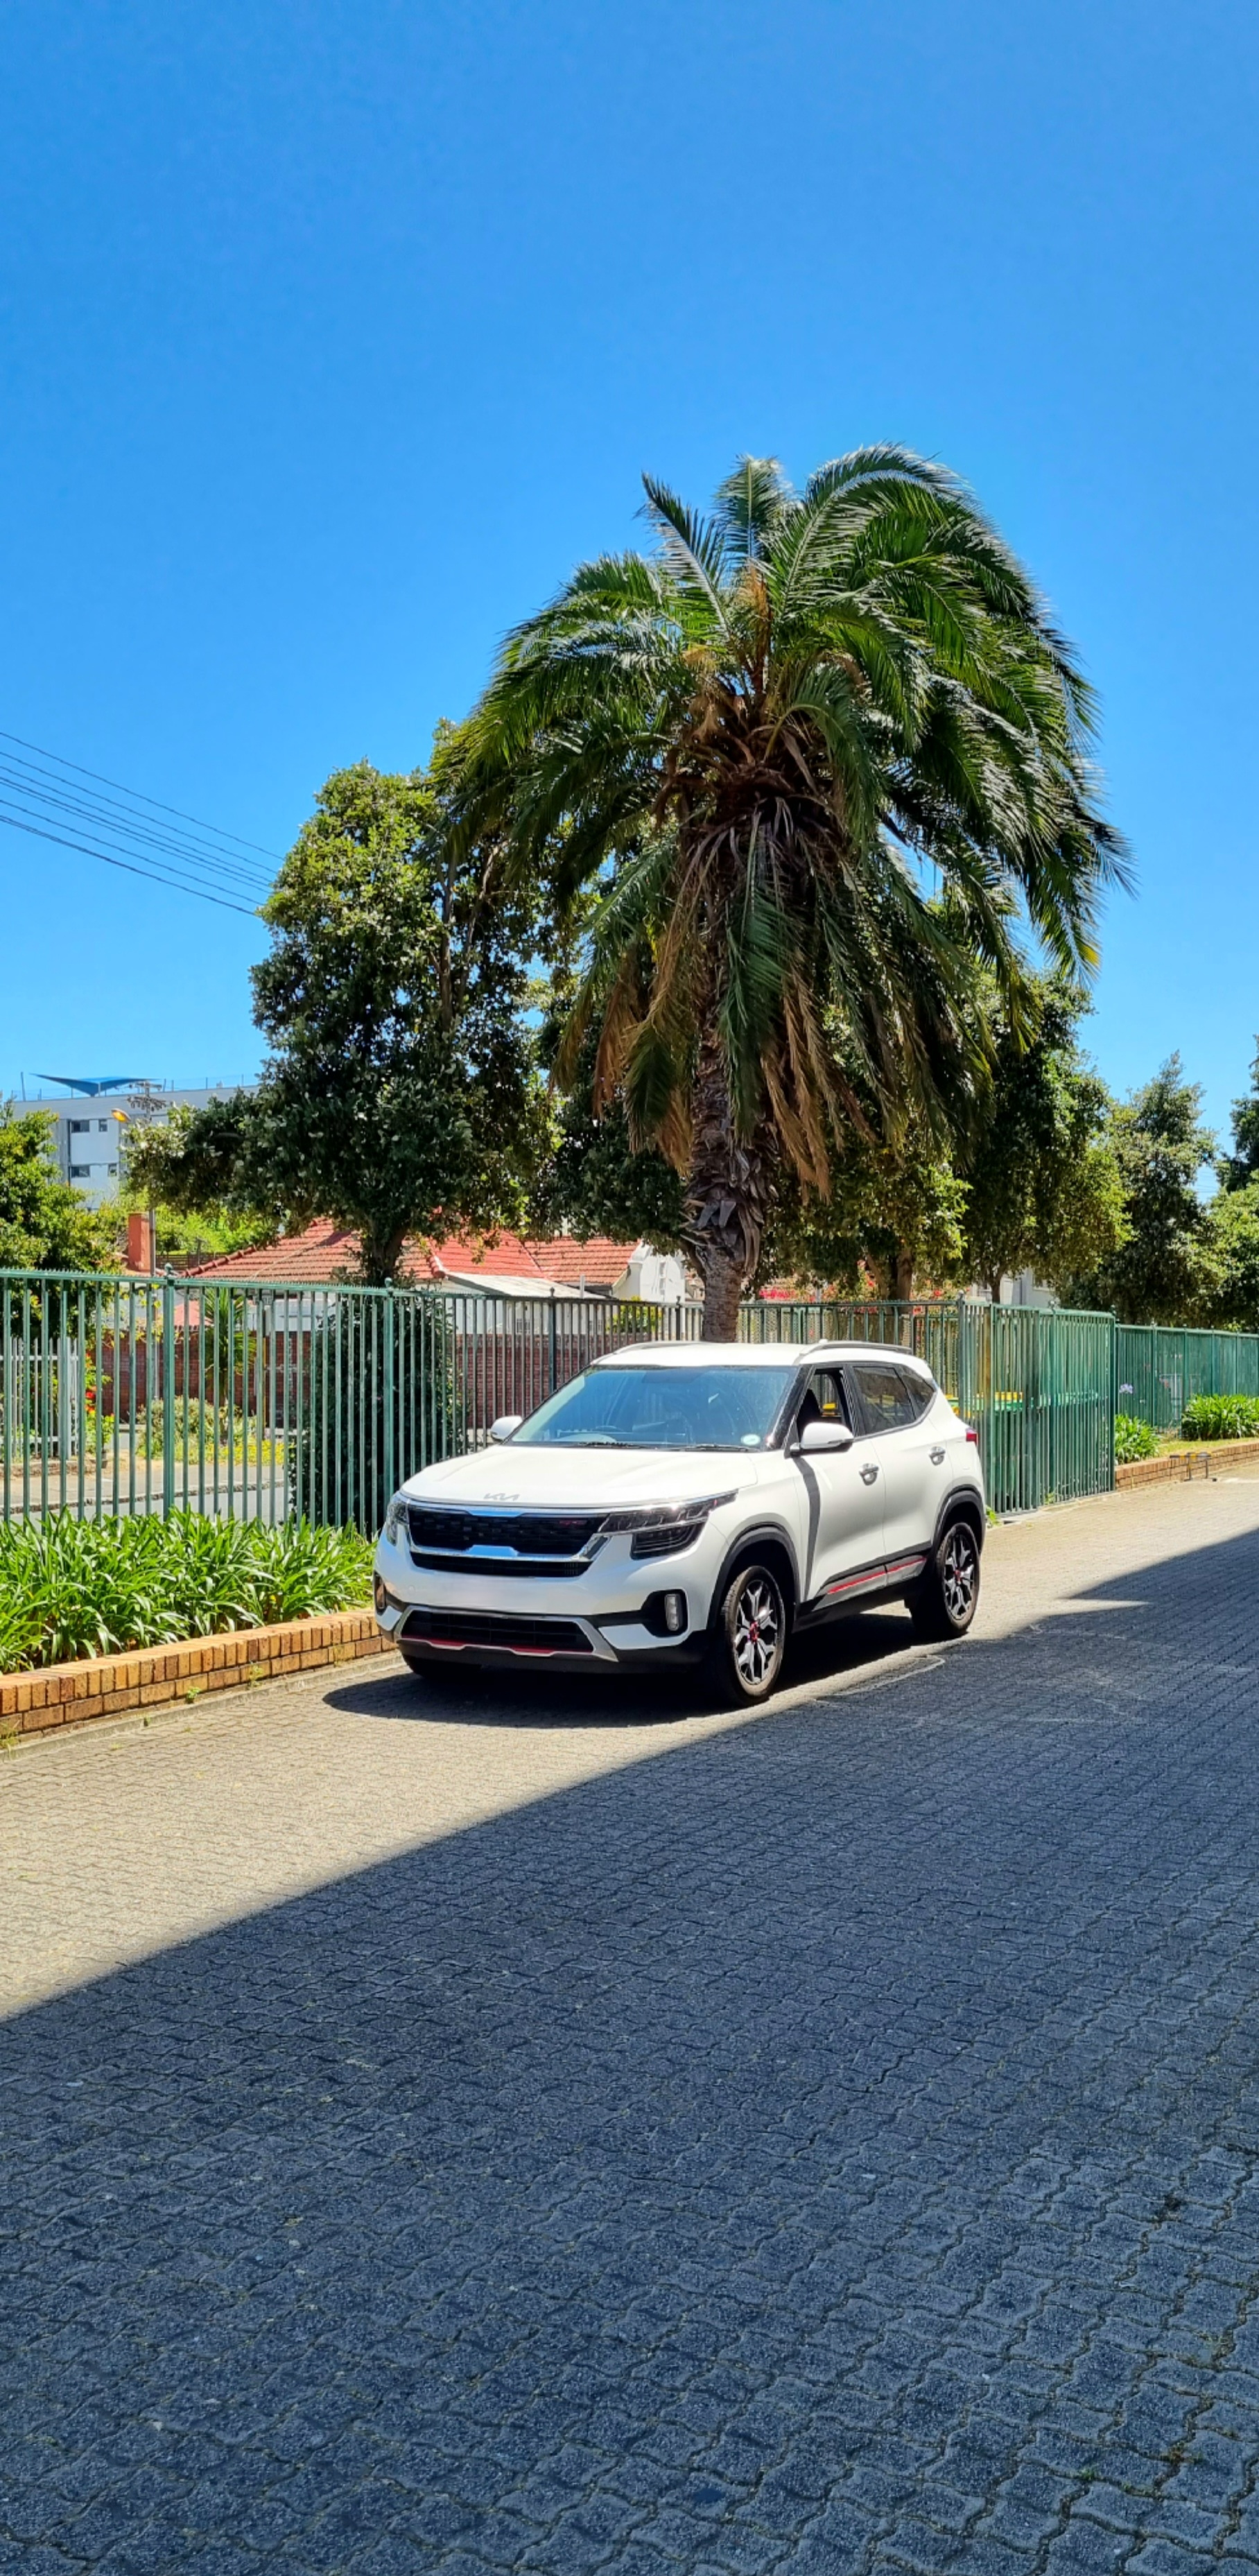
\includegraphics[width=6cm,height=6cm]{../Images/vehicles/1.jpg}}
        \caption{Vehicle 1.}
    \end{subfigure}
    ~ 
        \begin{subfigure}[t]{0.4\textwidth}
        \centering
        \def\svgwidth{1\linewidth}
        {\scriptsize
            \setstretch{0.7} % Line spacing
            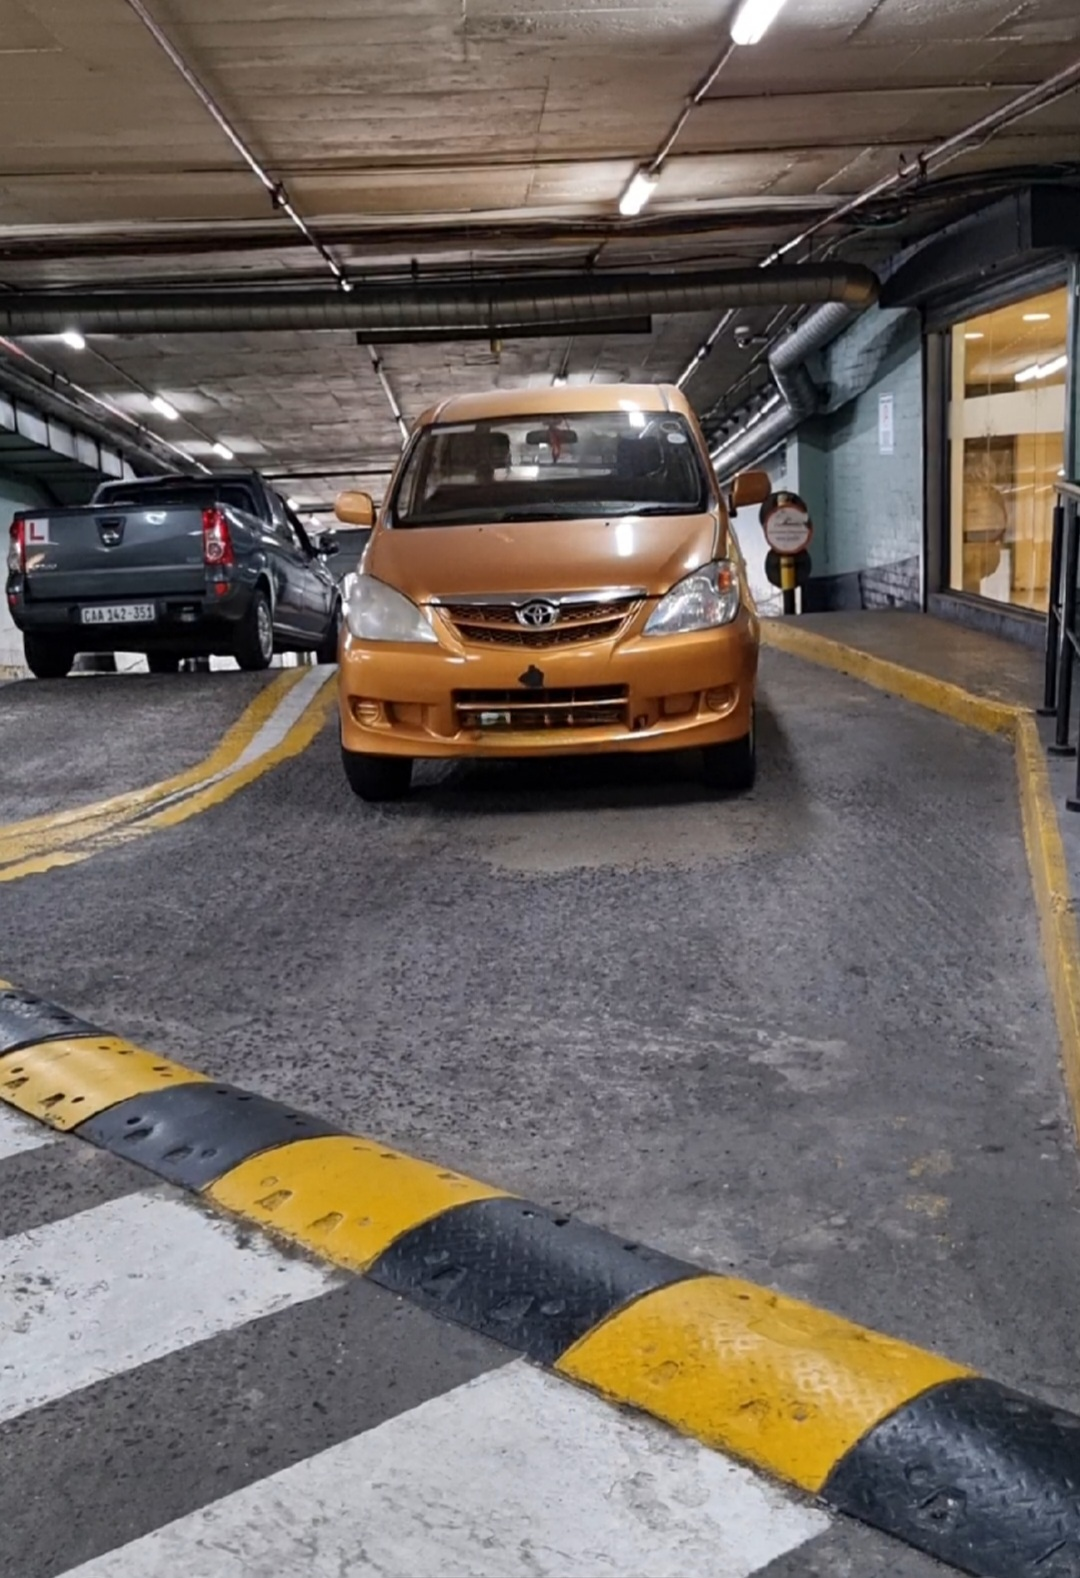
\includegraphics[width=6cm,height=6cm]{../Images/vehicles/2.jpg}}
        \caption{Vehicle 2.}
    \end{subfigure}
    ~     \begin{subfigure}[t]{0.4\textwidth}
        \centering
        \def\svgwidth{1\linewidth}
        {\scriptsize
            \setstretch{0.7} % Line spacing
            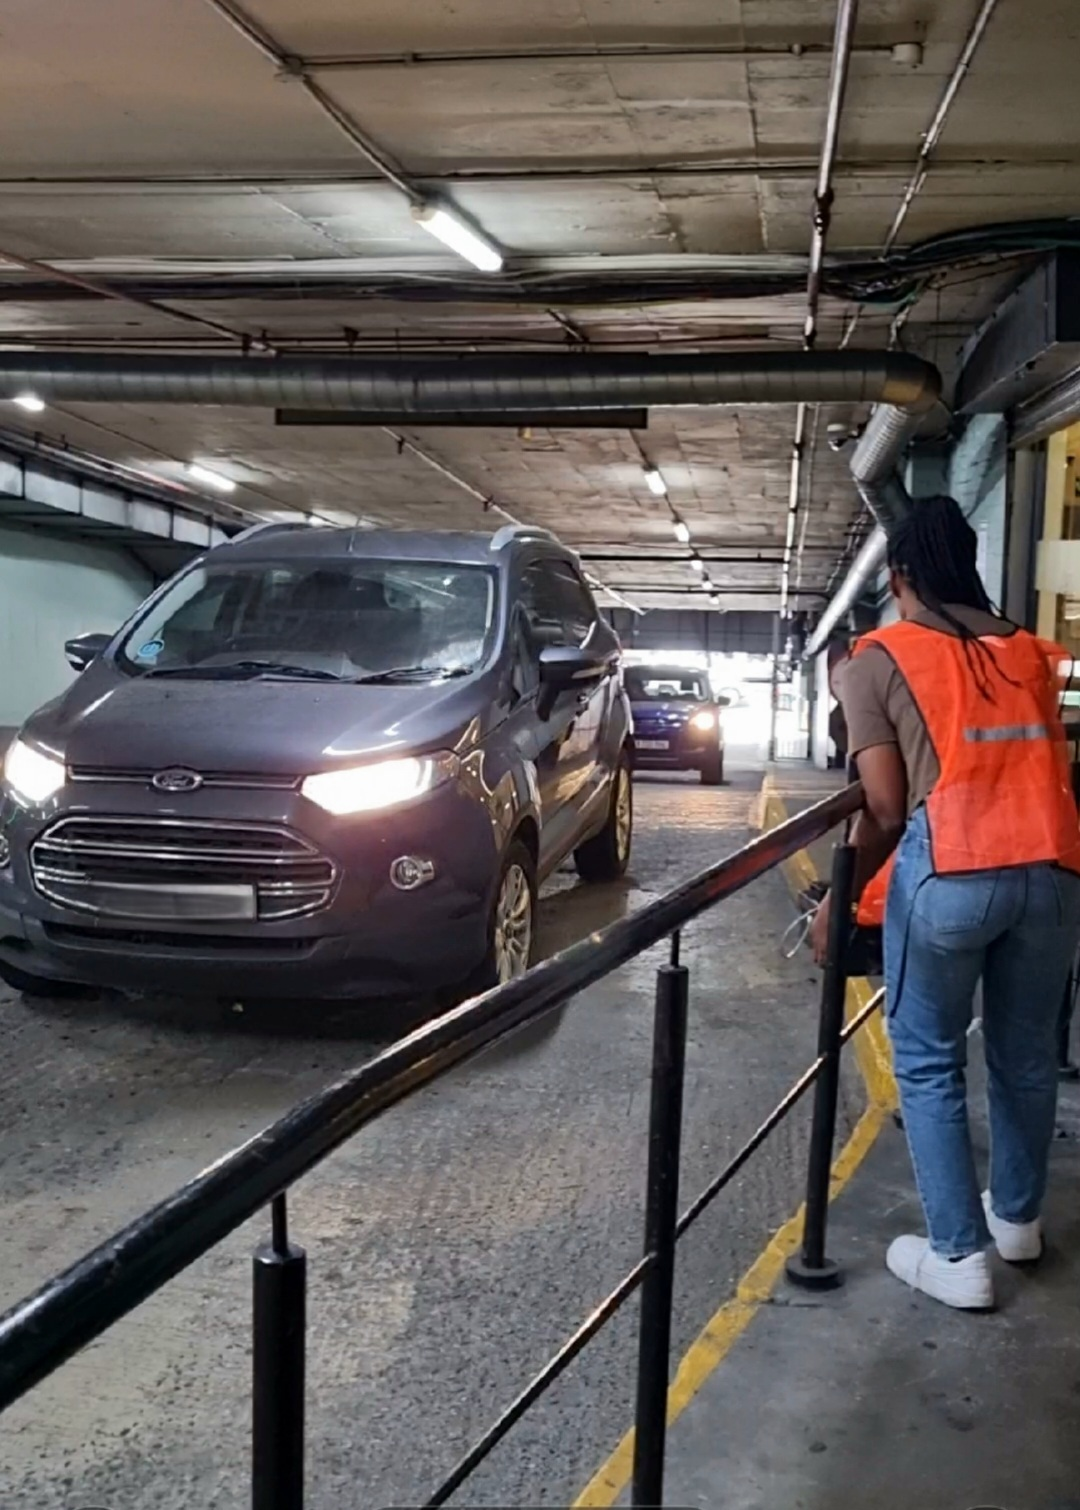
\includegraphics[width=6cm,height=6cm]{../Images/vehicles/3.jpg}}
        \caption{Vehicle 3.}
    \end{subfigure}
    ~     \begin{subfigure}[t]{0.4\textwidth}
        \centering
        \def\svgwidth{1\linewidth}
        {\scriptsize
            \setstretch{0.7} % Line spacing
            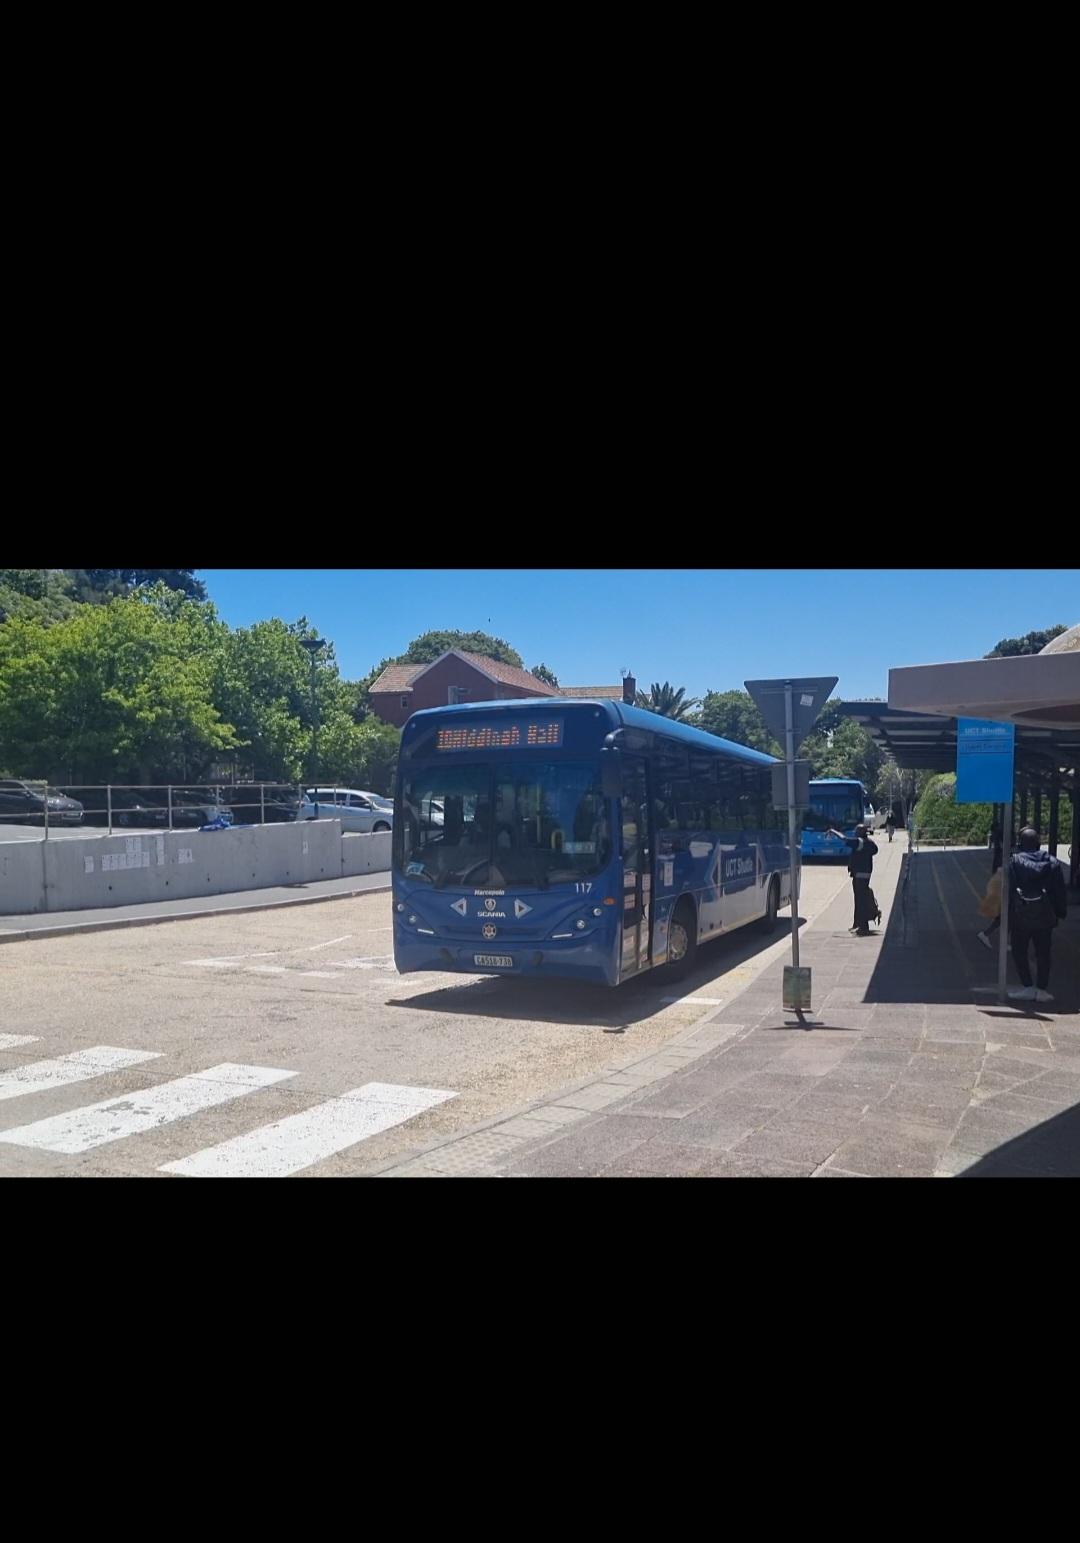
\includegraphics[width=6cm,height=6cm]{../Images/vehicles/4.jpg}}
        \caption{Vehicle 4.}
    \end{subfigure}
    ~     \begin{subfigure}[t]{0.4\textwidth}
        \centering
        \def\svgwidth{1\linewidth}
        {\scriptsize
            \setstretch{0.7} % Line spacing
            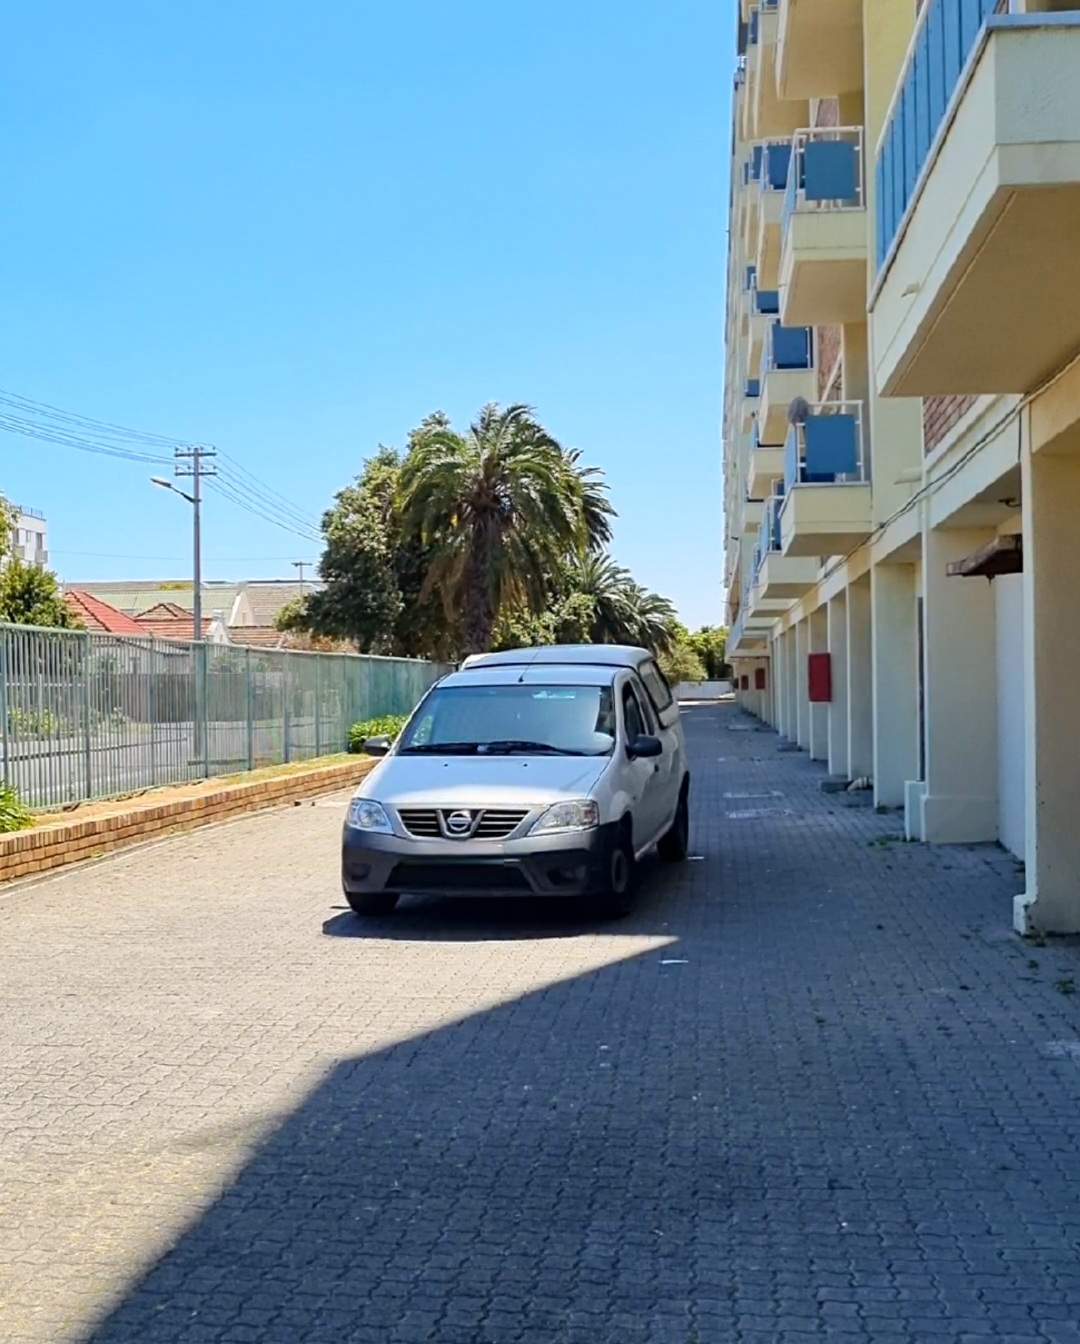
\includegraphics[width=6cm,height=6cm]{../Images/vehicles/5.jpg}}
        \caption{Vehicle 5.}
    \end{subfigure}
    \caption{Some vehicles used for experiments.}
\end{figure}

\section{Speed}
From the results in Table~\ref{tab:results}, it's not hard to notice that the speed values are off. In the case of the second and third small-to-medium car values, the speed recorded by the car's speedometer was 40 km/h and 18 km/h, respectively. These values do not correlate to that recorded by the demonstrator. This could, in effect, be an error on the side of the circuit, or an effect of incorrect signal processing techniques. However, the demonstrator is able to pick up the moving vehicle and provide a speed for the data collected.

\section{Range}
The range to the target is calculated using Equation~\ref{eqn:range} and the results displayed in Table~\ref{tab:range}.
\begin{table}[!htp]
\centering
\caption{\label{tab:range} Range to target vehicles.}
\vspace{-0.5cm}
\begin{tabular}{|m{5em}|m{5em}|}
\multicolumn{2}{l}{}\\
\cline{1-2}
Car type & Range (m) \\ \cline{1-2}
Small-to-medium car  & 41.16\\ \cline{1-2}
Small-to-medium car   & 10.87 \\ \cline{1-2}
Small-to-medium car   &  9.02\\ \cline{1-2}
Small-to-medium car   & 10.07\\ \cline{1-2}
Small-to-medium car   & 10.14\\ \cline{1-2}
Motorcycle  &  10.08\\ \cline{1-2}
Bus   & 10.07\\ \cline{1-2}
Bus   & 9.91\\ \cline{1-2}
\end{tabular}
\end{table}
The values in Table~\ref{tab:range} are surprisingly accurate to the distance values shown in Table~\ref{tab:results}. These values can be deemed as satisfactory for this work.

\section{Vehicle Size}
A look at Table~\ref{tab:vehicle-sizes} and Table~\ref{tab:range} will show that the demonstrator is capable of detecting vehicles of varying sizes, including motorcycles, small-to-medium size vehicles and busses. This aligns with the earlier prediction that objects with a larger \gls{rcs} will be more detectable by the demonstrator. This shows that the demonstrator is satisfactory for detecting larger size objects such as vehicles.
% ----------------------------------------------------
\ifstandalone
\bibliography{../Bibliography/References.bib}
\printnoidxglossary[type=\acronymtype,nonumberlist]
\fi
\end{document}
% ----------------------------------------------------